% begin module linear-functions
\begin{frame}
\frametitle{Linear Functions}
\begin{definition}[Linear Function]
A linear function is a function the graph of which is a line.  We can write any linear function in slope-intercept form:
\[
f(x) = mx + b.
\]
$m$ is called the slope, and $b$ is called the $y$-intercept.
\end{definition}
\end{frame}

\begin{frame}
\begin{columns}[c]
\column{.5\textwidth}
\ \only<handout:0| -2>{%
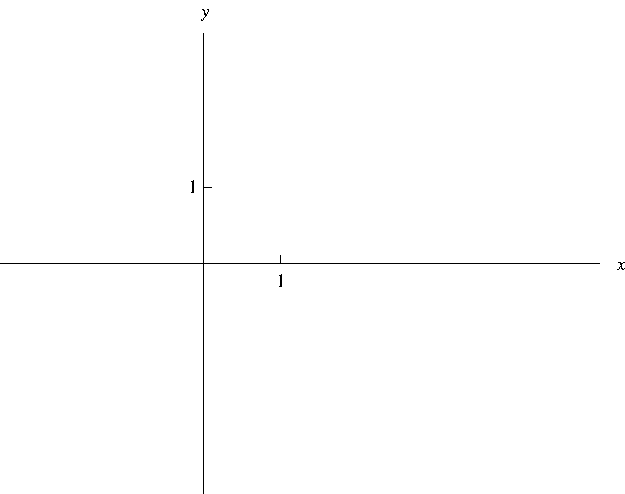
\includegraphics[height=4.5cm]{precalculus/pictures/01-02-linesa.pdf}%
}%
\only<handout:0| 3>{%
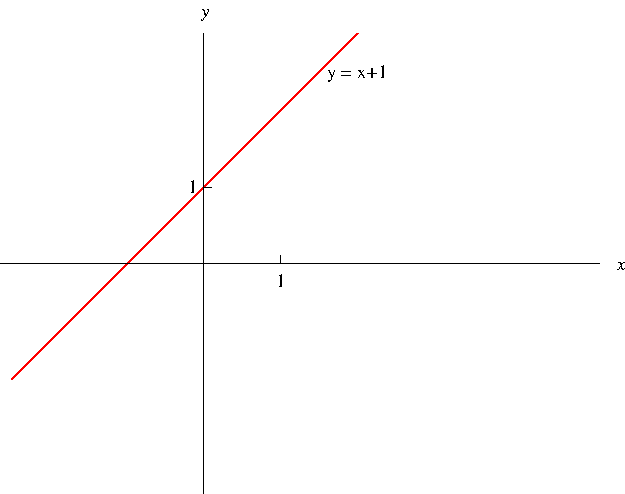
\includegraphics[height=4.5cm]{precalculus/pictures/01-02-linesb.pdf}%
}%
\only<handout:0| 4>{%
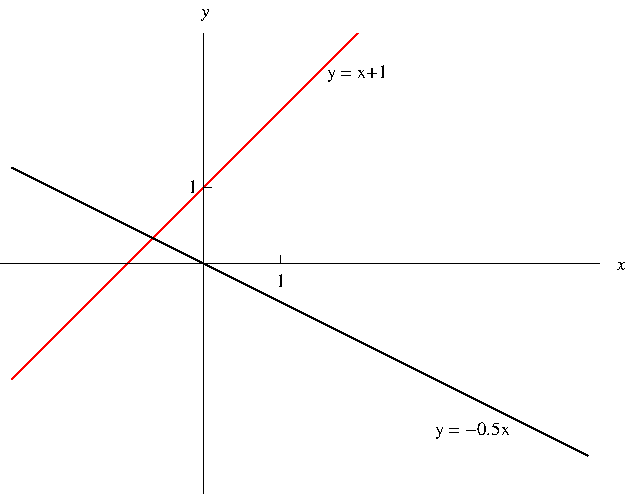
\includegraphics[height=4.5cm]{precalculus/pictures/01-02-linesc.pdf}%
}%
\only<handout:0| 5>{%
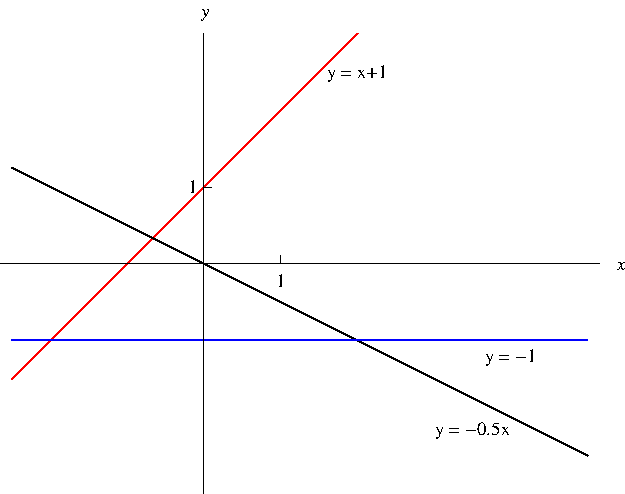
\includegraphics[height=4.5cm]{precalculus/pictures/01-02-linesd.pdf}%
}%
\only<handout:0| 6>{%
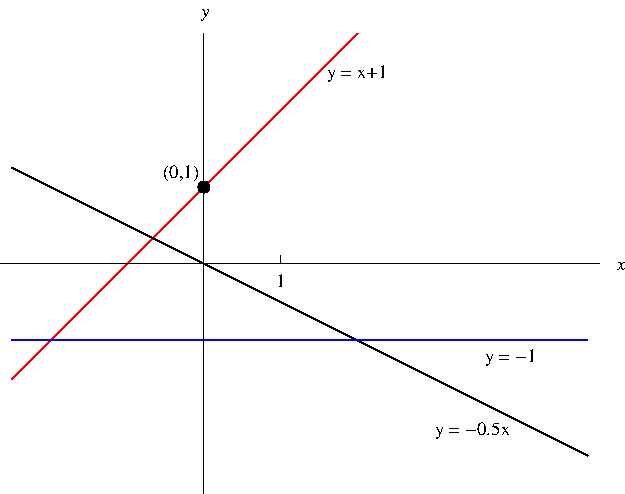
\includegraphics[height=4.5cm]{precalculus/pictures/01-02-linese.pdf}%
}%
\only<handout:0| 7>{%
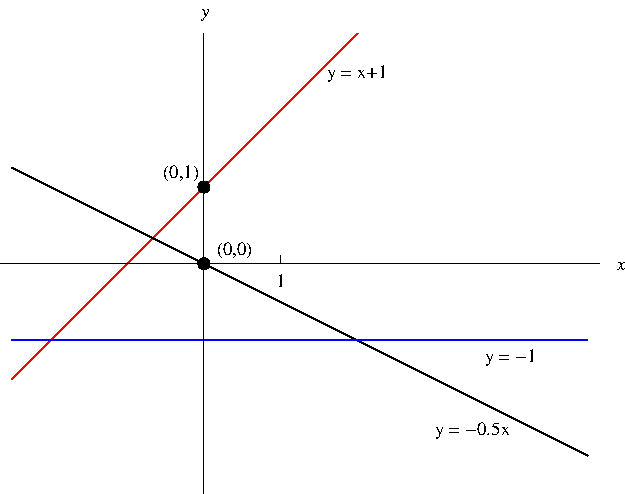
\includegraphics[height=4.5cm]{precalculus/pictures/01-02-linesf.pdf}%
}%
\only<8>{%
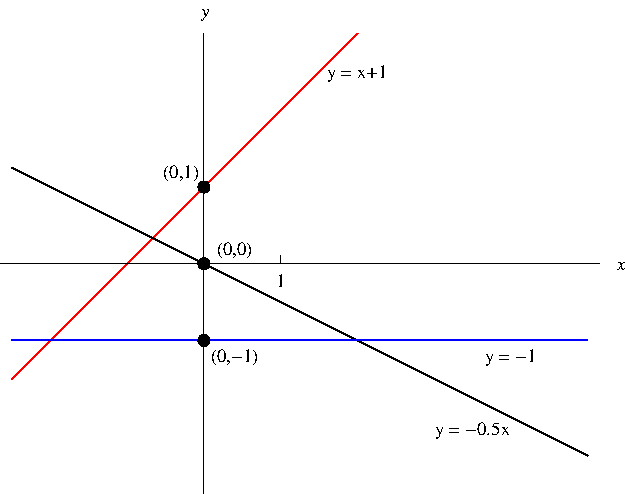
\includegraphics[height=4.5cm]{precalculus/pictures/01-02-linesg.pdf}%
}%
\column[t]{.55\textwidth}
\begin{tabular}{|c|c|c|}
\hline
$f(x)$ & Direction & $y$-intercept \\
\hline
\uncover<3->{\alert<handout:0| 3>{$x + \alert<handout:0| 6>{1}$}} & 
\uncover<3->{\alert<handout:0| 3>{$\nearrow$}} & 
\uncover<6->{\alert<handout:0| 6>{1}} \\
\uncover<4->{\alert<handout:0| 4>{$-0.5x \uncover<7>{\alert<handout:0| 7>{+ 0}}$}} & 
\uncover<4->{\alert<handout:0| 4>{$\searrow$}} & 
\uncover<7->{\alert<handout:0| 7>{0}} \\
\uncover<5->{\alert<handout:0| 5,8>{$-1$}} & 
\uncover<5->{\alert<handout:0| 5>{$\rightarrow$}} & 
\uncover<8->{\alert<handout:0| 8>{-1}} \\
\hline
\end{tabular}
\end{columns}

\begin{itemize}
\item<3->  $m > 0$ means the graph of $f$ points up ($\nearrow$).
\item<4->  $m < 0$ means the graph of $f$ points down ($\searrow$).
\item<5->  $m = 0$ means the graph of $f$ is horizontal ($\rightarrow$).
\item<6->  $b$ tells us the height of the point where the graph hits the $y$-axis.
\end{itemize}
\end{frame}
% end module linear-functions
